\section{Makefile}
A construção do nosso Makefile foi rápida e teve poucos problemas. conseguimos entender rápidamente a estrutura simples.
\begin{verbatim}
[Arquivo a ser gerado] : [Dependências - Arquivos que servem como fonte]
    [O código que deve ser executado pelo terminal]
\end{verbatim}
Tivemos alguns problemas com o TAB, que precisa necessariamente ter 4 espaços. Nós usamos o editor Atom que tem o TAB configurado como 2 espaços. Alteramos isso, e nosso Makefile funcionou perfeitamente.
\par Posteriormente tivemos problemas, que a priori achamos que fosse no código, mas logo percebemos que era no Makefile: toda vez que alteravamos o código para testes de chars para ints ou vice versa, o programa não executava da forma esperada. Depois de quase dois dias revisando, percebemos que nosso .h não é compilado, mas ele é usado em todos os nossos .c. Quando mudamos o tipo da váriavel alteramos o .h, mas apenas alguns .c, fazendo com que alguns .c fiquem com o .h antigo e outros com o novo. Resolvemos isso simplesmente adicionando o .h como dependência de todos os .o, como visto no exemplo abaixo:

\begin{figure}[!h]
\centering
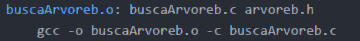
\includegraphics[width=5in]{relatorio/imagens/imgMakefile.png}
\end{figure}

\par Isso foi tudo que fizemos com o Makefile. Na próxima seção discutiremos sobre a inserção.